\subsubsection{Text preprocessing}
\label{sub:text_preprocessing}

In general, neural networks require numerical inputs, i.e., scalars or vectors.
For example, images can be processed by looking at pixel values representing
coloration, which can either be scalar (grey-scale image) or multi-dimensional
(RGB image).
Consequently, in order to include tweet texts as input to a neural network,
the respective texts need to be transformed into numbers.
This is usually achieved by obtaining vector representations for single words.
Such a mapping between words and vectors of real numbers is called a \textbf{word
embedding}.
This section is structured as follows.
First, an introduction to word vectors are given.
Afterwards, all five steps of the transformation process are be presented using a simple example.
In addition, intermediate results of the preprocessing steps for the collected
data sets are described.
The example used throughout this section comprises two fictional tweet texts:

\begin{enumerate}
  \item Tweet: ``The weather is so niceee!!! \#ILoveDarmstadt''
  \item Tweet: ``@rogerfederer is an 8 time Wimbledon champion! \#achievement''
\end{enumerate}

These will be preprocessed so that they can be used as an actual input to a neural network.

\paragraph{Word vectors}
\label{sub:word_vectors}

As mentioned above, an embedding is a function that maps from a specific
vocabulary to vectors with dimensionality $d$.
As a results, words are effectively placed in a vector space $\mathbb{R}^d$.
This allows examination of space structure and relationships between words of 
the vocabulary.
This thesis uses the pre-trained \textit{GloVe} word vectors by the \textit{Stanford
Natural Language Processing Group}\footcite{Pennington2014}\footnote{\url{https://nlp.stanford.edu/projects/glove/}}.
These were trained on a corpus of two billion tweets containing a total of
27 billion unique token from different languages, e.g., English, Arabic and
Japanese.
Here, a token can be a word or a symbol with a special meaning.
In detail, vectors were obtained by examining co-occurrence statistics in this
large data set.
Two special featues come with this set of word vectors.
Firstly, it is possible to quantify linguistic or semantic similarity between
words by calculating the Euclidian distance between them.
For example, the word pair ``frog-toad'' should have a smaller distance than
the pair ``frog-tiger'', because frogs and toads are both amphibians.
Secondly, calculating semantic distance allow to compare relatedness of word
pairs, so-called linear substructures.
As an example, the word pair ``man-woman'' should intuitively have similar distance
compared to the pair ``king-queen'', since the underlying concept to distinguish
the words is gender.
Using pre-existing word vectors removes the need to learn these parameters
at training time, thus speeding up the model development process.

\paragraph{Tokenization}
\label{sub:tokenization}

Making maximum use of pre-trained word vectors requires preprocessing the raw
tweet texts so that they are in conformity with existing standards set by
the creators.
Explicitly, \textit{GloVe} word vectors come with predefined tokens for tweet
components such as hashtags, URLs or user mentions, stylistic expressions such
as punctuation repetition or word elongation, and general concepts like numbers.
These tokens need to be recognized and marked in tweet texts.
In addtion, tokenization should preprocess the texts in a way that they can
later be separated into single tokens by simply splitting on whitespace.

\begin{table}
\begin{tabular}{rlll}
\toprule
Step & Description & Before & After \\
\midrule
1 & Mark URLs & ``https://t.co/IFt05'' & ``<url>'' \\
2 & Split words separated by slashes & ``fruits/vegetables'' & ``fruits / vegetables'' \\
3 & Mark user mentions & ``@rogerfederer'' & ``<user>'' \\
4 & Mark emoticons & ``:-)'' & ``<smile>'' \\
5 & Mark numbers & ``123'' & ``<number>'' \\
6 & Mark and split hashtags & ``\#SoNice'' & ``<hashtag> so nice'' \\
7 & Mark punctuation repetitions & ``!!!'' & ``! <repeat>'' \\
8 & Add spaces around punctuation & ``Watch out!'' & ``watch out !'' \\
9 & Mark elongated words & ``niceeeee'' & ``nice <elong>'' \\
10 & Mark allcaps words & ``IMPORTANT'' & ``important <allcaps>'' \\
11 & Remove unicode character & ``u00B3'' & `` '' \\
\bottomrule
\end{tabular}
\caption{Order of text preprocessing steps}
\label{tab:text_preprocessing}
\end{table}

Table~\ref{tab:text_preprocessing} shows the undertaken tweet preprocessing
steps for this thesis.
These are inspired by a Ruby script written by the GloVe creators\footnote{\url{https://nlp.stanford.edu/projects/glove/preprocess-twitter.rb}}.
The code was ported to Python, including necessary fixes and expansions.
Special tokens often replace the original content, e.g., for URLs, user mentions,
numbers and emoticons.
The main reason behind this is that consuming algorithms are more capable of
making sense of the general occurrence of such components, rather than their
actual meaning.
For example, a neural network will not be able to derive the content of the
actual web pages behind URLs.
Stylistic expressions such as word elongations, punctuation repetitions or
allcaps words could be useful to learn about tweet sentiment since the author is 
obviously trying to highlight the specific passage.
Words that are transformed, e.g., by elongations or uppercasing, are converted to their original, lowercase
version for easier matching with the pre-trained word vectors.
Since hashtags are often written in camelcase form, they are split on uppercase
letters with the aim of understanding the meaning behind them.
Finally, spaces are added where needed, e.g., between slashes (obviously after
replacing URLs) or around punctuation.

\begin{figure}[h]
  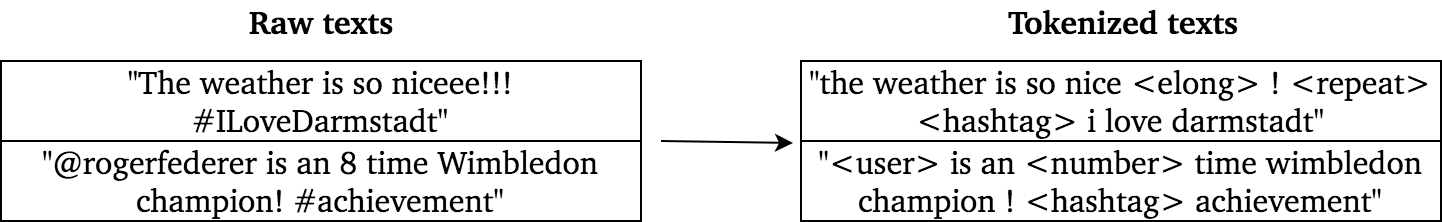
\includegraphics[width=\textwidth]{img/text_preprocessing_1}
  \caption{Tokenization example}
\label{fig:tokenization}
\end{figure}

Fig.~\ref{fig:tokenization} presents the results of applying the above listed
steps to the example tweets used in this section.
The tokenized texts are prepared for the next preprocessing steps, which
are described in the following paragraphs.
In practice, the derived tokenizations are often noisy due to individual tweeting
behaviors.
Unconvential writing often leads to the creation of unknown tokens and other
edge cases which are not covered by pre-trained word vectors.
This constitutes one of the reasons why huge amounts of data are usually needed
for NLP tasks.

\paragraph{Word index}
\label{sub:word_index}

The next step of creating a word embedding is to compile a list of all unique
words (resp.\ tokens) in the data set.
As a results, the word index is developed, which constitutes a map structure.
Here the words serve as keys, and the values are unique, numerical identifiers
(IDs) for these words.

\begin{figure}[h]
  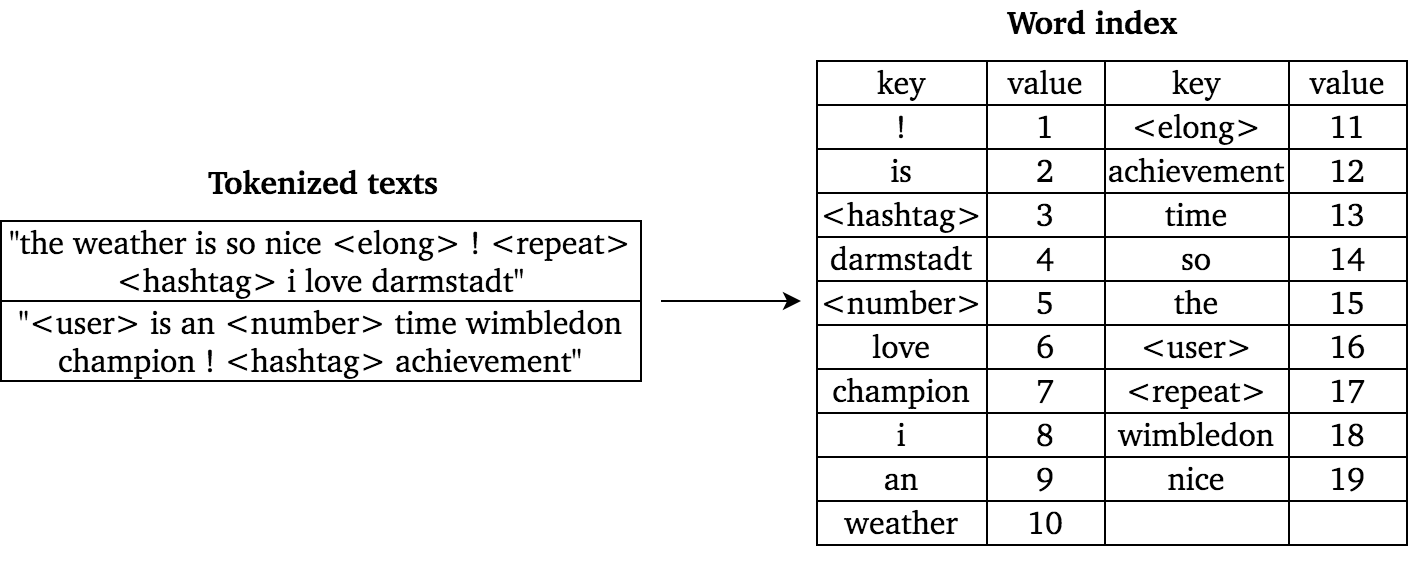
\includegraphics[width=\textwidth]{img/text_preprocessing_2}
  \caption{Word index example}
\label{fig:word_index}
\end{figure}

Fig.~\ref{fig:word_index} shows the resulting word index for the simple
example.
In this case, the word index contains a total of 19 words.
The word IDs are usually ordered according to the number of occurrences of the
associated word.
In this example, exclamation mark, the word ``is'' and the hashtag token occur
twice and are therefore given the smallest IDs.
Ordering words in this way enables straightforward separation of the most
popular words, if the vocabulary for further examination is restricted for some
reason (e.g., computational ressources are limited).
It is important to note, that word IDs should be ascending with step size 1 and
start at 1.
The reasons for that will become obvious in the following paragraphs.

Applying this procedure to the collected data sets results in the creation of
word indices, whose sizes differ considerably.
More precisely, totals of 34,295 (celebrity tweets), 56,265 (politician tweets),
98,027 (company tweets) and 225,171 (combined set of tweets) words are identified.
Unsurprisingly, the most commonly occurring tokens across all data sets are markers
for URLs, hashtags and users, punctuation like full stop and exclamation mark,
definite and indefinite articles, as well as prepositions like ``to'', ``for''
and ``of''.

\paragraph{Sequences}
\label{sub:sequences}

At this stage, the input texts can be transformed into sequences, i.e., lists
of word IDs.
This step requires tokenized texts and a complete word index, both of which
are available at this point.

\begin{figure}[h]
  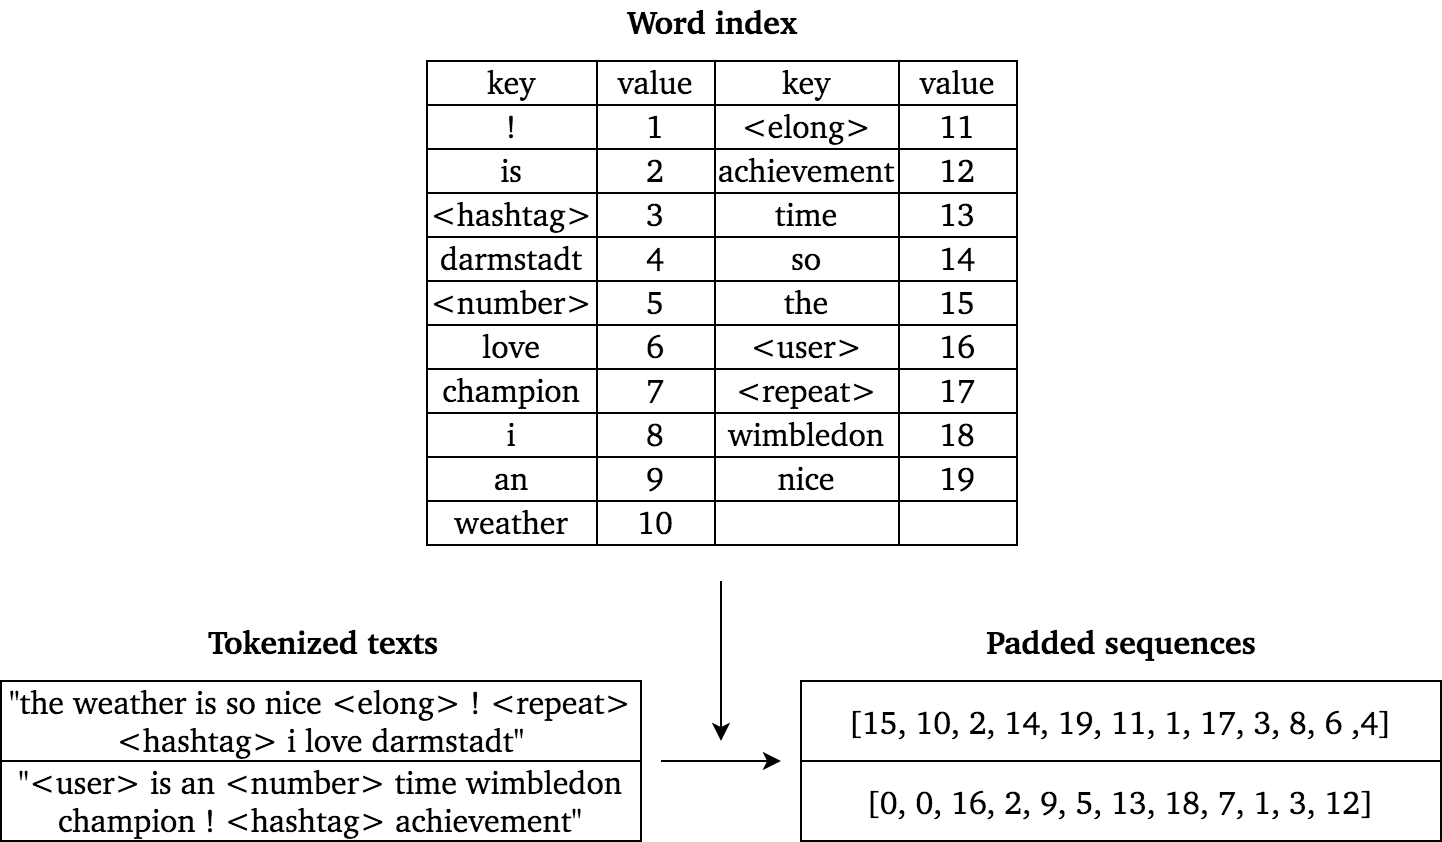
\includegraphics[width=\textwidth]{img/text_preprocessing_3}
  \caption{Text sequencing example}
\label{fig:text_sequencing}
\end{figure}

The result of sequencing the example tweets is illustrated in Fig.~\ref{fig:text_sequencing}.
Firstly, tokenized texts are split into a list of tokens.
Split points can usually be defined tailored to the specific problem, but
most commonly input texts are split on any kind of whitespace, i.e., spaces,
tabs or newlines.
Secondly, the list entries are transformed from actual words to their respective
word IDs.
This happens via a simple lookup in the word index.
To recap, word indices are usually implemented as map structures, which are
optimized for these kinds of lookup procedures.
The resulting sequences possess varying lengths, due to the variation of the
underlying texts.
As a third and final step, the sequences are padded so that the differences in
length vanish.
This is achieved by either inserting zero values or removing sequence entries,
depending on the specified common length.
Often the longest sequence determines this common length, but it can also be
set to an arbitrary number (e.g., if particular outliers in length exist).
In this example, the second sequence is padded with two leading zeros.
For the collected data sets, sequence lengths were set to 32 or 48, which
means at least 99\% of all tweets were considered in full length.

\paragraph{Embedding index}
\label{sub:embedding_index}

The word index basically defines the vocabulary used in the input texts.
Contained words now have to be equipped with word vectors, so that the
consuming algorithm can make sense of this data.
In this thesis, pre-trained word vectors are utilized, which come in form of a
simple text file.
The next step of creating a word embedding is to load the vectors from file
into a more conveniently accessible data structure, thus creating the so-called
\textit{embedding index}.

\begin{figure}[h]
  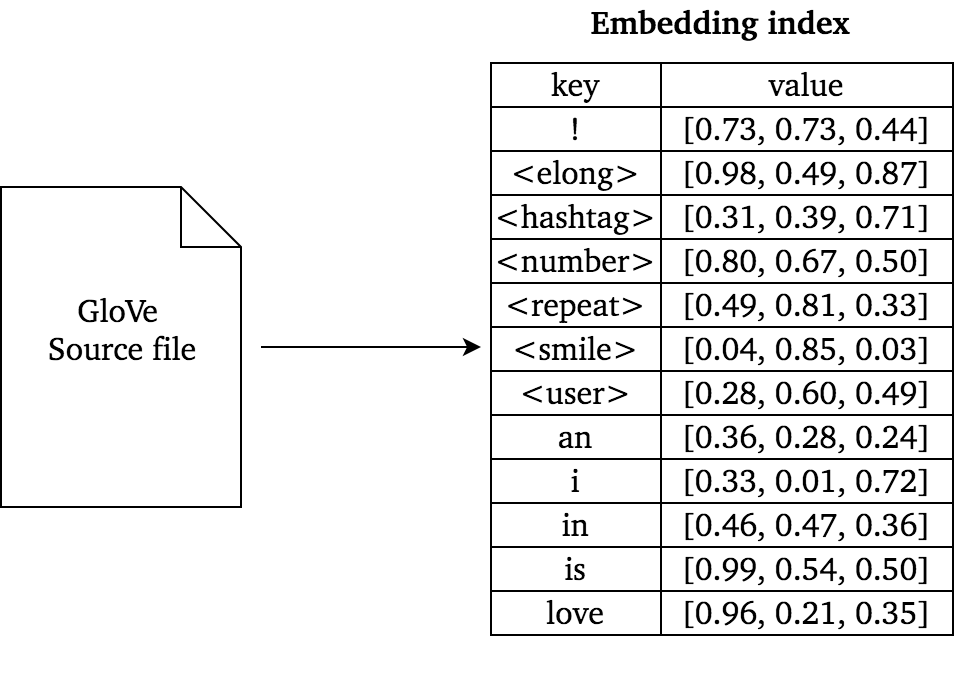
\includegraphics[height=7cm]{img/text_preprocessing_4}
  \caption{Embedding index example}
\label{fig:embedding_index}
\end{figure}

Fig.~\ref{fig:embedding_index} shows how the embedding index typically looks
like.
In accordance to the word index, the embedding index is most commonly implemented
as a map structure (e.g., \textit{dictionaries} in Python).
Once again, the particular word serves as a unique key for lookups.
Loaded word vectors are assigned as values.
Vectors are usually represented as lists of some kind, e.g., arrays in Python.
Vector dimensionality is predetermined, e.g., GloVe comes with vectors of length
25, 50, 100 and 200.
In this example, a random three-dimensional representation is chosen for more
improved overview.
Moreover, it is assumed that the pre-trained vectors only cover a very restricted
vocabulary.
Generally, it should be denoted that using pre-trained word vectors does not guarantee
to derive numerical representations for every token in the word index.
How this problem is dealt with will be outlined in the upcoming paragraph.

\paragraph{Embedding matrix}
\label{sub:embedding_matrix}

The ultimate goal of creating an word embedding is to derive the so-called
\textit{embedding matrix}, which serves as an initial weight matrix for the
embedding layer in a neural network.
Thus, the final step of the text preprocessing process is to derive this
matrix in which the $i^{th}$ row represents the word vector for word with ID $i$
in the word index.
As a results, the embedding layer can iterate over input sequences and simply
replace word IDs with vector one at a time.
The dimensionality of the embedding matrix is then given by the length of the
word index (number of rows) and chosen vector dimensionality $d$ (number of columns).

\begin{figure}[h]
  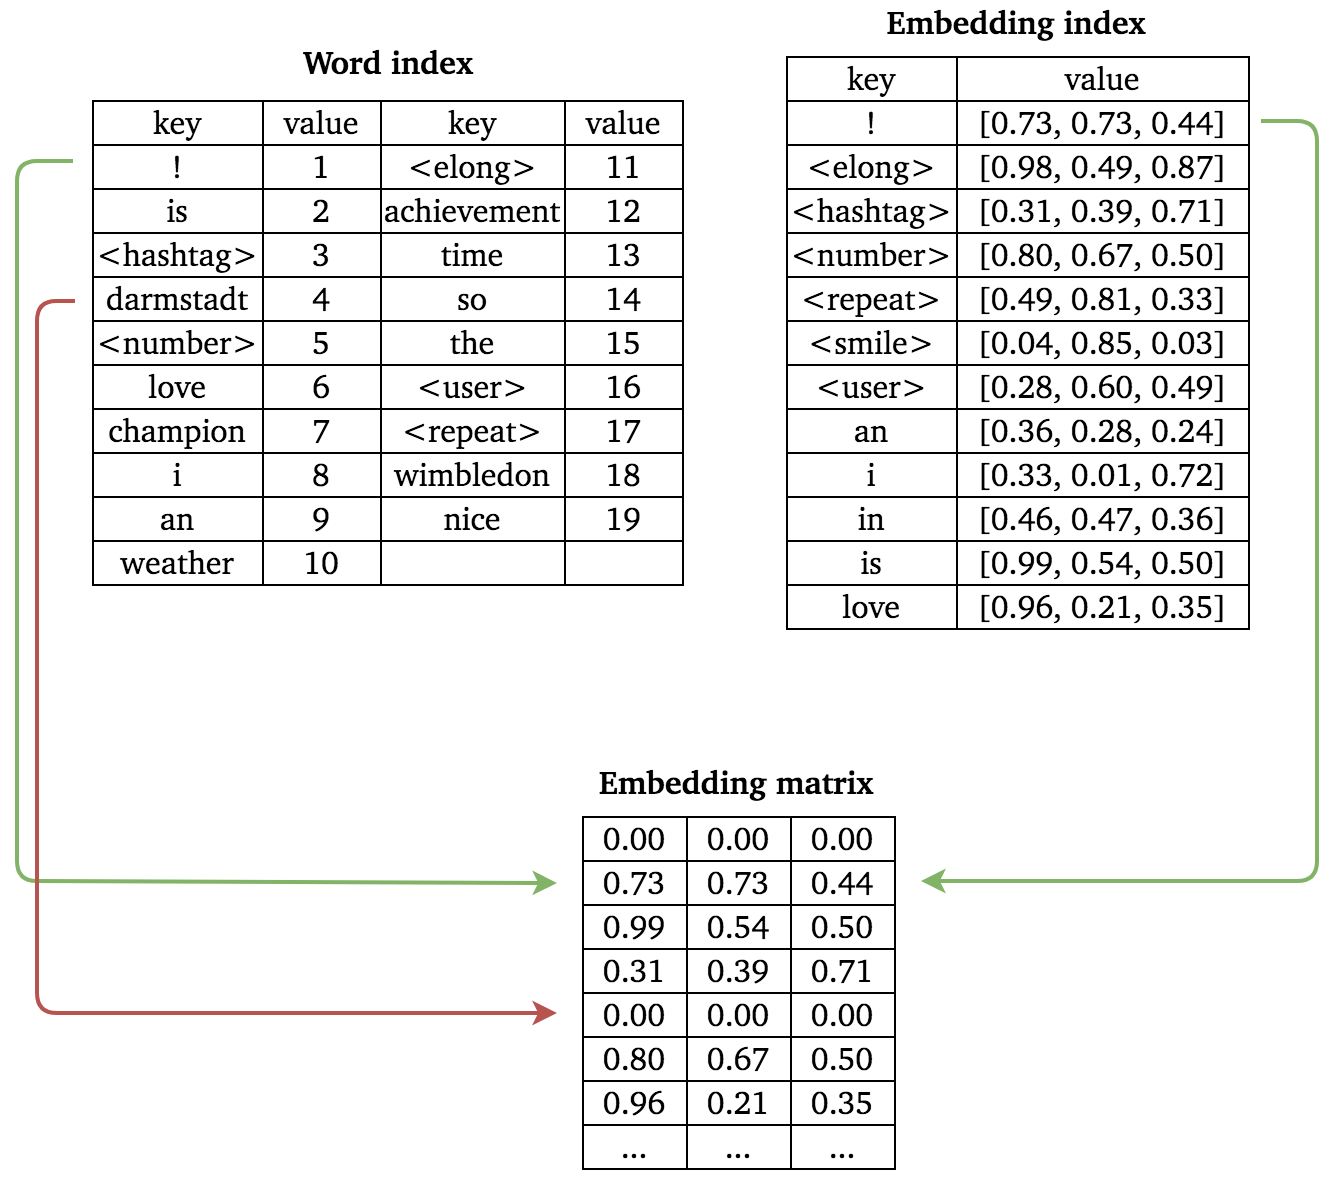
\includegraphics[width=\textwidth]{img/text_preprocessing_5}
  \caption{Embedding matrix example}
\label{fig:embedding_matrix}
\end{figure}

Fig.~\ref{fig:embedding_matrix} illustrates the creation process of the embedding
matrix for the running example.
In detail, the embedding matrix is created by iterating over the word index.
For each key, it is checked whether an entry with the same key exists in the
embedding index.
If this is the case, the $i^{th}$ row of the embedding matrix is filled with
the derived word vector.
In Fig.~\ref{fig:embedding_matrix}, this successful lookup is shown for the
exclamation mark token, denoted by the green arrows.
Contrary, if a mismatch between input and word vector vocabularies exists, i.e.,
no matching word vector is found in the embedding index, the respective row
is filled with zeros.
In this example, this is the case for the ``darmstadt'' token, signified by the
red arrow.

Creating the embedding matrix completes necessary text preprocessing.
Word and embedding index serve as intermediate results, which might be helpful
for analyzing model results.
Embedding matrix and padded sequences are directly used in the consuming
algorithm, here a deep neural network.
Detailed explications about their usage as model components can be found in the
following section which presents architectures of the developed models.
